%! TEX program = pdflatex
\documentclass[a4paper]{article}
\usepackage{amsmath,amssymb}
\usepackage{amsmath}
\usepackage{graphicx}
\usepackage{tikz}
\usepackage[top=3cm, bottom=3cm, left=2.54cm, right=2.54cm]{geometry}
\usepackage{fancyhdr}
\pagestyle{fancy}

\definecolor{blueceu}{RGB}{5,161,230}

\lhead{\textsc{\color{blueceu}{CEU San Pablo University}}} \rhead{\textsl{\textsf{\color{blueceu}Department of Applied Maths and Statistics}}}
\renewcommand{\headrulewidth}{0pt}
\renewcommand{\floatpagefraction}{.8}
\renewcommand{\textfraction}{.1}

\begin{document}

\section*{\color{blueceu}Standard Normal Distribution Function $\boldsymbol Z\sim N(0,1)$}
\begin{center}
\scalebox{0.6}{
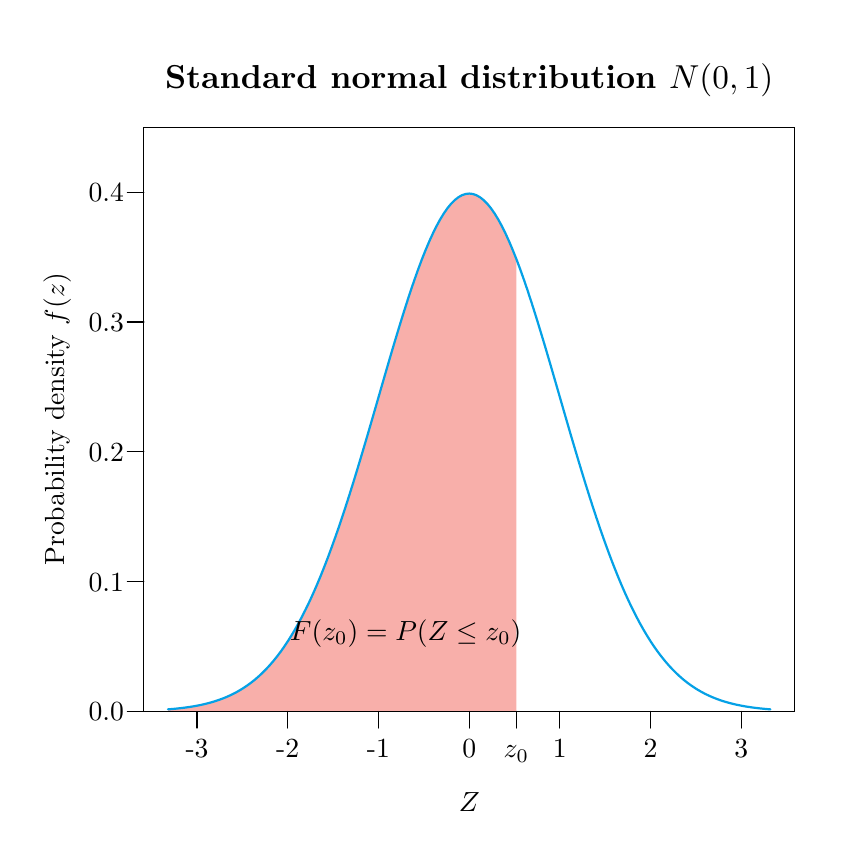
\begin{tikzpicture}[x=1pt,y=1pt]
  \definecolor{fillColor}{RGB}{255,255,255}
  \path[use as bounding box,fill=fillColor,fill opacity=0.00] (0,0) rectangle (289.08,289.08);
  \begin{scope}
  \path[clip] (  0.00,  0.00) rectangle (289.08,289.08);
  \definecolor{drawColor}{RGB}{0,0,0}
  
  \path[draw=drawColor,line width= 0.4pt,line join=round,line cap=round] ( 61.20, 42.00) -- (257.88, 42.00);
  
  \path[draw=drawColor,line width= 0.4pt,line join=round,line cap=round] ( 61.20, 42.00) -- ( 61.20, 36.00);
  
  \path[draw=drawColor,line width= 0.4pt,line join=round,line cap=round] ( 93.98, 42.00) -- ( 93.98, 36.00);
  
  \path[draw=drawColor,line width= 0.4pt,line join=round,line cap=round] (126.76, 42.00) -- (126.76, 36.00);
  
  \path[draw=drawColor,line width= 0.4pt,line join=round,line cap=round] (159.54, 42.00) -- (159.54, 36.00);
  
  \path[draw=drawColor,line width= 0.4pt,line join=round,line cap=round] (192.32, 42.00) -- (192.32, 36.00);
  
  \path[draw=drawColor,line width= 0.4pt,line join=round,line cap=round] (225.10, 42.00) -- (225.10, 36.00);
  
  \path[draw=drawColor,line width= 0.4pt,line join=round,line cap=round] (257.88, 42.00) -- (257.88, 36.00);
  
  \node[text=drawColor,anchor=base,inner sep=0pt, outer sep=0pt, scale=  1.00] at ( 61.20, 25.20) {-3};
  
  \node[text=drawColor,anchor=base,inner sep=0pt, outer sep=0pt, scale=  1.00] at ( 93.98, 25.20) {-2};
  
  \node[text=drawColor,anchor=base,inner sep=0pt, outer sep=0pt, scale=  1.00] at (126.76, 25.20) {-1};
  
  \node[text=drawColor,anchor=base,inner sep=0pt, outer sep=0pt, scale=  1.00] at (159.54, 25.20) {0};
  
  \node[text=drawColor,anchor=base,inner sep=0pt, outer sep=0pt, scale=  1.00] at (192.32, 25.20) {1};
  
  \node[text=drawColor,anchor=base,inner sep=0pt, outer sep=0pt, scale=  1.00] at (225.10, 25.20) {2};
  
  \node[text=drawColor,anchor=base,inner sep=0pt, outer sep=0pt, scale=  1.00] at (257.88, 25.20) {3};
  
  \path[draw=drawColor,line width= 0.4pt,line join=round,line cap=round] ( 42.00, 42.00) -- ( 42.00,229.63);
  
  \path[draw=drawColor,line width= 0.4pt,line join=round,line cap=round] ( 42.00, 42.00) -- ( 36.00, 42.00);
  
  \path[draw=drawColor,line width= 0.4pt,line join=round,line cap=round] ( 42.00, 88.91) -- ( 36.00, 88.91);
  
  \path[draw=drawColor,line width= 0.4pt,line join=round,line cap=round] ( 42.00,135.81) -- ( 36.00,135.81);
  
  \path[draw=drawColor,line width= 0.4pt,line join=round,line cap=round] ( 42.00,182.72) -- ( 36.00,182.72);
  
  \path[draw=drawColor,line width= 0.4pt,line join=round,line cap=round] ( 42.00,229.63) -- ( 36.00,229.63);
  
  \node[text=drawColor,anchor=base east,inner sep=0pt, outer sep=0pt, scale=  1.00] at ( 34.80, 38.56) {0.0};
  
  \node[text=drawColor,anchor=base east,inner sep=0pt, outer sep=0pt, scale=  1.00] at ( 34.80, 85.46) {0.1};
  
  \node[text=drawColor,anchor=base east,inner sep=0pt, outer sep=0pt, scale=  1.00] at ( 34.80,132.37) {0.2};
  
  \node[text=drawColor,anchor=base east,inner sep=0pt, outer sep=0pt, scale=  1.00] at ( 34.80,179.28) {0.3};
  
  \node[text=drawColor,anchor=base east,inner sep=0pt, outer sep=0pt, scale=  1.00] at ( 34.80,226.18) {0.4};
  
  \path[draw=drawColor,line width= 0.4pt,line join=round,line cap=round] ( 42.00, 42.00) --
    (277.08, 42.00) --
    (277.08,253.08) --
    ( 42.00,253.08) --
    ( 42.00, 42.00);
  \end{scope}
  \begin{scope}
  \path[clip] (  0.00,  0.00) rectangle (289.08,289.08);
  \definecolor{drawColor}{RGB}{0,0,0}
  
  \node[text=drawColor,anchor=base,inner sep=0pt, outer sep=0pt, scale=  1.20] at (159.54,266.94) {\bfseries Standard normal distribution $N(0,1)$};
  
  \node[text=drawColor,anchor=base,inner sep=0pt, outer sep=0pt, scale=  1.00] at (159.54,  6.00) {$Z$};
  
  \node[text=drawColor,rotate= 90.00,anchor=base,inner sep=0pt, outer sep=0pt, scale=  1.00] at ( 13.20,147.54) {Probability density $f(z)$};
  \end{scope}
  \begin{scope}
  \path[clip] (  0.00,  0.00) rectangle (289.08,289.08);
  \definecolor{drawColor}{RGB}{0,0,0}
  
  \path[draw=drawColor,line width= 0.4pt,line join=round,line cap=round] (176.59, 42.00) -- (176.59, 42.00);
  
  \path[draw=drawColor,line width= 0.4pt,line join=round,line cap=round] (176.59, 42.00) -- (176.59, 36.00);
  
  \node[text=drawColor,anchor=base,inner sep=0pt, outer sep=0pt, scale=  1.00] at (176.59, 25.20) {$z_0$};
  \end{scope}
  \begin{scope}
  \path[clip] ( 42.00, 42.00) rectangle (277.08,253.08);
  \definecolor{fillColor}{RGB}{238,50,36}
  
  \path[fill=fillColor,fill opacity=0.39] ( 50.71, 42.00) --
    ( 50.71, 42.76) --
    ( 52.02, 42.86) --
    ( 53.33, 42.98) --
    ( 54.64, 43.12) --
    ( 55.95, 43.27) --
    ( 57.26, 43.44) --
    ( 58.57, 43.63) --
    ( 59.89, 43.84) --
    ( 61.20, 44.08) --
    ( 62.51, 44.34) --
    ( 63.82, 44.63) --
    ( 65.13, 44.96) --
    ( 66.44, 45.32) --
    ( 67.75, 45.71) --
    ( 69.06, 46.15) --
    ( 70.38, 46.63) --
    ( 71.69, 47.16) --
    ( 73.00, 47.74) --
    ( 74.31, 48.37) --
    ( 75.62, 49.06) --
    ( 76.93, 49.82) --
    ( 78.24, 50.64) --
    ( 79.55, 51.54) --
    ( 80.87, 52.50) --
    ( 82.18, 53.55) --
    ( 83.49, 54.69) --
    ( 84.80, 55.91) --
    ( 86.11, 57.23) --
    ( 87.42, 58.64) --
    ( 88.73, 60.16) --
    ( 90.04, 61.78) --
    ( 91.36, 63.51) --
    ( 92.67, 65.36) --
    ( 93.98, 67.33) --
    ( 95.29, 69.41) --
    ( 96.60, 71.62) --
    ( 97.91, 73.96) --
    ( 99.22, 76.43) --
    (100.53, 79.03) --
    (101.85, 81.77) --
    (103.16, 84.63) --
    (104.47, 87.63) --
    (105.78, 90.76) --
    (107.09, 94.03) --
    (108.40, 97.42) --
    (109.71,100.95) --
    (111.02,104.59) --
    (112.34,108.35) --
    (113.65,112.23) --
    (114.96,116.22) --
    (116.27,120.30) --
    (117.58,124.48) --
    (118.89,128.75) --
    (120.20,133.09) --
    (121.51,137.49) --
    (122.83,141.94) --
    (124.14,146.44) --
    (125.45,150.96) --
    (126.76,155.50) --
    (128.07,160.04) --
    (129.38,164.56) --
    (130.69,169.05) --
    (132.00,173.50) --
    (133.32,177.88) --
    (134.63,182.19) --
    (135.94,186.40) --
    (137.25,190.50) --
    (138.56,194.48) --
    (139.87,198.30) --
    (141.18,201.97) --
    (142.49,205.47) --
    (143.81,208.77) --
    (145.12,211.87) --
    (146.43,214.74) --
    (147.74,217.39) --
    (149.05,219.79) --
    (150.36,221.94) --
    (151.67,223.82) --
    (152.98,225.43) --
    (154.30,226.75) --
    (155.61,227.79) --
    (156.92,228.53) --
    (158.23,228.98) --
    (159.54,229.13) --
    (160.85,228.98) --
    (162.16,228.53) --
    (163.47,227.79) --
    (164.78,226.75) --
    (166.10,225.43) --
    (167.41,223.82) --
    (168.72,221.94) --
    (170.03,219.79) --
    (171.34,217.39) --
    (172.65,214.74) --
    (173.96,211.87) --
    (175.27,208.77) --
    (176.59,205.47) --
    (176.59, 42.00) --
    cycle;
  \definecolor{drawColor}{RGB}{5,161,230}
  
  \path[draw=drawColor,line width= 0.8pt,line join=round,line cap=round] ( 50.71, 42.76) --
    ( 52.02, 42.86) --
    ( 53.33, 42.98) --
    ( 54.64, 43.12) --
    ( 55.95, 43.27) --
    ( 57.26, 43.44) --
    ( 58.57, 43.63) --
    ( 59.89, 43.84) --
    ( 61.20, 44.08) --
    ( 62.51, 44.34) --
    ( 63.82, 44.63) --
    ( 65.13, 44.96) --
    ( 66.44, 45.32) --
    ( 67.75, 45.71) --
    ( 69.06, 46.15) --
    ( 70.38, 46.63) --
    ( 71.69, 47.16) --
    ( 73.00, 47.74) --
    ( 74.31, 48.37) --
    ( 75.62, 49.06) --
    ( 76.93, 49.82) --
    ( 78.24, 50.64) --
    ( 79.55, 51.54) --
    ( 80.87, 52.50) --
    ( 82.18, 53.55) --
    ( 83.49, 54.69) --
    ( 84.80, 55.91) --
    ( 86.11, 57.23) --
    ( 87.42, 58.64) --
    ( 88.73, 60.16) --
    ( 90.04, 61.78) --
    ( 91.36, 63.51) --
    ( 92.67, 65.36) --
    ( 93.98, 67.33) --
    ( 95.29, 69.41) --
    ( 96.60, 71.62) --
    ( 97.91, 73.96) --
    ( 99.22, 76.43) --
    (100.53, 79.03) --
    (101.85, 81.77) --
    (103.16, 84.63) --
    (104.47, 87.63) --
    (105.78, 90.76) --
    (107.09, 94.03) --
    (108.40, 97.42) --
    (109.71,100.95) --
    (111.02,104.59) --
    (112.34,108.35) --
    (113.65,112.23) --
    (114.96,116.22) --
    (116.27,120.30) --
    (117.58,124.48) --
    (118.89,128.75) --
    (120.20,133.09) --
    (121.51,137.49) --
    (122.83,141.94) --
    (124.14,146.44) --
    (125.45,150.96) --
    (126.76,155.50) --
    (128.07,160.04) --
    (129.38,164.56) --
    (130.69,169.05) --
    (132.00,173.50) --
    (133.32,177.88) --
    (134.63,182.19) --
    (135.94,186.40) --
    (137.25,190.50) --
    (138.56,194.48) --
    (139.87,198.30) --
    (141.18,201.97) --
    (142.49,205.47) --
    (143.81,208.77) --
    (145.12,211.87) --
    (146.43,214.74) --
    (147.74,217.39) --
    (149.05,219.79) --
    (150.36,221.94) --
    (151.67,223.82) --
    (152.98,225.43) --
    (154.30,226.75) --
    (155.61,227.79) --
    (156.92,228.53) --
    (158.23,228.98) --
    (159.54,229.13) --
    (160.85,228.98) --
    (162.16,228.53) --
    (163.47,227.79) --
    (164.78,226.75) --
    (166.10,225.43) --
    (167.41,223.82) --
    (168.72,221.94) --
    (170.03,219.79) --
    (171.34,217.39) --
    (172.65,214.74) --
    (173.96,211.87) --
    (175.27,208.77) --
    (176.59,205.47) --
    (177.90,201.97) --
    (179.21,198.30) --
    (180.52,194.48) --
    (181.83,190.50) --
    (183.14,186.40) --
    (184.45,182.19) --
    (185.76,177.88) --
    (187.08,173.50) --
    (188.39,169.05) --
    (189.70,164.56) --
    (191.01,160.04) --
    (192.32,155.50) --
    (193.63,150.96) --
    (194.94,146.44) --
    (196.25,141.94) --
    (197.57,137.49) --
    (198.88,133.09) --
    (200.19,128.75) --
    (201.50,124.48) --
    (202.81,120.30) --
    (204.12,116.22) --
    (205.43,112.23) --
    (206.74,108.35) --
    (208.06,104.59) --
    (209.37,100.95) --
    (210.68, 97.42) --
    (211.99, 94.03) --
    (213.30, 90.76) --
    (214.61, 87.63) --
    (215.92, 84.63) --
    (217.23, 81.77) --
    (218.55, 79.03) --
    (219.86, 76.43) --
    (221.17, 73.96) --
    (222.48, 71.62) --
    (223.79, 69.41) --
    (225.10, 67.33) --
    (226.41, 65.36) --
    (227.72, 63.51) --
    (229.04, 61.78) --
    (230.35, 60.16) --
    (231.66, 58.64) --
    (232.97, 57.23) --
    (234.28, 55.91) --
    (235.59, 54.69) --
    (236.90, 53.55) --
    (238.21, 52.50) --
    (239.53, 51.54) --
    (240.84, 50.64) --
    (242.15, 49.82) --
    (243.46, 49.06) --
    (244.77, 48.37) --
    (246.08, 47.74) --
    (247.39, 47.16) --
    (248.70, 46.63) --
    (250.02, 46.15) --
    (251.33, 45.71) --
    (252.64, 45.32) --
    (253.95, 44.96) --
    (255.26, 44.63) --
    (256.57, 44.34) --
    (257.88, 44.08) --
    (259.19, 43.84) --
    (260.51, 43.63) --
    (261.82, 43.44) --
    (263.13, 43.27) --
    (264.44, 43.12) --
    (265.75, 42.98) --
    (267.06, 42.86) --
    (268.37, 42.76);
  \definecolor{drawColor}{RGB}{0,0,0}
  
  \node[text=drawColor,anchor=base,inner sep=0pt, outer sep=0pt, scale=  1.00] at (136.59, 67.64) {$F(z_0)=P(Z\leq z_0)$};
  \end{scope}
  \begin{scope}
  \path[clip] (  0.00,  0.00) rectangle (289.08,289.08);
  \definecolor{drawColor}{RGB}{0,0,0}
  
  \path[draw=drawColor,line width= 0.4pt,line join=round,line cap=round] ( 42.00, 42.00) --
    (277.08, 42.00) --
    (277.08,253.08) --
    ( 42.00,253.08) --
    ( 42.00, 42.00);
  \end{scope}
  \end{tikzpicture}
}
\end{center}

\begin{center}
\begin{tabular}
{|r||r|r|r|r|r|r|r|r|r|r|}
\hline
\multicolumn{1}{|c||}{$\mathbf{z}$}&
\multicolumn{1}{c|}{\textbf{0,00}}&
\multicolumn{1}{c|}{\textbf{0,01}}&
\multicolumn{1}{c|}{\textbf{0,02}}&
\multicolumn{1}{c|}{\textbf{0,03}}&
\multicolumn{1}{c|}{\textbf{0,04}}&
\multicolumn{1}{c|}{\textbf{0,05}}&
\multicolumn{1}{c|}{\textbf{0,06}}&
\multicolumn{1}{c|}{\textbf{0,07}}&
\multicolumn{1}{c|}{\textbf{0,08}}&
\multicolumn{1}{c|}{\textbf{0,09}}\\
\hline\hline
\textbf{-3,4}&
0,0003&
0,0003&
0,0003&
0,0003&
0,0003&
0,0003&
0,0003&
0,0003&
0,0003&
0,0002 \\
\hline
\textbf{-3,3}&
0,0005&
0,0005&
0,0005&
0,0004&
0,0004&
0,0004&
0,0004&
0,0004&
0,0004&
0,0003 \\
\hline
\textbf{-3,2}&
0,0007&
0,0007&
0,0006&
0,0006&
0,0006&
0,0006&
0,0006&
0,0005&
0,0005&
0,0005 \\
\hline
\textbf{-3,1}&
0,0010&
0,0009&
0,0009&
0,0009&
0,0008&
0,0008&
0,0008&
0,0008&
0,0007&
0,0007 \\
\hline
\textbf{-3,0}&
0,0013&
0,0013&
0,0013&
0,0012&
0,0012&
0,0011&
0,0011&
0,0011&
0,0010&
0,0010 \\
\hline
\textbf{-2,9}&
0,0019&
0,0018&
0,0018&
0,0017&
0,0016&
0,0016&
0,0015&
0,0015&
0,0014&
0,0014 \\
\hline
\textbf{-2,8}&
0,0026&
0,0025&
0,0024&
0,0023&
0,0023&
0,0022&
0,0021&
0,0021&
0,0020&
0,0019 \\
\hline
\textbf{-2,7}&
0,0035&
0,0034&
0,0033&
0,0032&
0,0031&
0,0030&
0,0029&
0,0028&
0,0027&
0,0026 \\
\hline
\textbf{-2,6}&
0,0047&
0,0045&
0,0044&
0,0043&
0,0041&
0,0040&
0,0039&
0,0038&
0,0037&
0,0036 \\
\hline
\textbf{-2,5}&
0,0062&
0,0060&
0,0059&
0,0057&
0,0055&
0,0054&
0,0052&
0,0051&
0,0049&
0,0048 \\
\hline
\textbf{-2,4}&
0,0082&
0,0080&
0,0078&
0,0075&
0,0073&
0,0071&
0,0069&
0,0068&
0,0066&
0,0064 \\
\hline
\textbf{-2,3}&
0,0107&
0,0104&
0,0102&
0,0099&
0,0096&
0,0094&
0,0091&
0,0089&
0,0087&
0,0084 \\
\hline
\textbf{-2,2}&
0,0139&
0,0136&
0,0132&
0,0129&
0,0125&
0,0122&
0,0119&
0,0116&
0,0113&
0,0110 \\
\hline
\textbf{-2,1}&
0,0179&
0,0174&
0,0170&
0,0166&
0,0162&
0,0158&
0,0154&
0,0150&
0,0146&
0,0143 \\
\hline
\textbf{-2,0}&
0,0228&
0,0222&
0,0217&
0,0212&
0,0207&
0,0202&
0,0197&
0,0192&
0,0188&
0,0183 \\
\hline
\textbf{-1,9}&
0,0287&
0,0281&
0,0274&
0,0268&
0,0262&
0,0256&
0,0250&
0,0244&
0,0239&
0,0233 \\
\hline
\textbf{-1,8}&
0,0359&
0,0351&
0,0344&
0,0336&
0,0329&
0,0322&
0,0314&
0,0307&
0,0301&
0,0294 \\
\hline
\textbf{-1,7}&
0,0446&
0,0436&
0,0427&
0,0418&
0,0409&
0,0401&
0,0392&
0,0384&
0,0375&
0,0367 \\
\hline
\textbf{-1,6}&
0,0548&
0,0537&
0,0526&
0,0516&
0,0505&
0,0495&
0,0485&
0,0475&
0,0465&
0,0455 \\
\hline
\textbf{-1,5}&
0,0668&
0,0655&
0,0643&
0,0630&
0,0618&
0,0606&
0,0594&
0,0582&
0,0571&
0,0559 \\
\hline
\textbf{-1,4}&
0,0808&
0,0793&
0,0778&
0,0764&
0,0749&
0,0735&
0,0721&
0,0708&
0,0694&
0,0681 \\
\hline
\textbf{-1,3}&
0,0968&
0,0951&
0,0934&
0,0918&
0,0901&
0,0885&
0,0869&
0,0853&
0,0838&
0,0823 \\
\hline
\textbf{-1,2}&
0,1151&
0,1131&
0,1112&
0,1093&
0,1075&
0,1056&
0,1038&
0,1020&
0,1003&
0,0985 \\
\hline
\textbf{-1,1}&
0,1357&
0,1335&
0,1314&
0,1292&
0,1271&
0,1251&
0,1230&
0,1210&
0,1190&
0,1170 \\
\hline
\textbf{-1,0}&
0,1587&
0,1562&
0,1539&
0,1515&
0,1492&
0,1469&
0,1446&
0,1423&
0,1401&
0,1379 \\
\hline
\textbf{-0,9}&
0,1841&
0,1814&
0,1788&
0,1762&
0,1736&
0,1711&
0,1685&
0,1660&
0,1635&
0,1611 \\
\hline
\textbf{-0,8}&
0,2119&
0,2090&
0,2061&
0,2033&
0,2005&
0,1977&
0,1949&
0,1922&
0,1894&
0,1867 \\
\hline
\textbf{-0,7}&
0,2420&
0,2389&
0,2358&
0,2327&
0,2296&
0,2266&
0,2236&
0,2206&
0,2177&
0,2148 \\
\hline
\textbf{-0,6}&
0,2743&
0,2709&
0,2676&
0,2643&
0,2611&
0,2578&
0,2546&
0,2514&
0,2483&
0,2451 \\
\hline
\textbf{-0,5}&
0,3085&
0,3050&
0,3015&
0,2981&
0,2946&
0,2912&
0,2877&
0,2843&
0,2810&
0,2776 \\
\hline
\textbf{-0,4}&
0,3446&
0,3409&
0,3372&
0,3336&
0,3300&
0,3264&
0,3228&
0,3192&
0,3156&
0,3121 \\
\hline
\textbf{-0,3}&
0,3821&
0,3783&
0,3745&
0,3707&
0,3669&
0,3632&
0,3594&
0,3557&
0,3520&
0,3483 \\
\hline
\textbf{-0,2}&
0,4207&
0,4168&
0,4129&
0,4090&
0,4052&
0,4013&
0,3974&
0,3936&
0,3897&
0,3859 \\
\hline
\textbf{-0,1}&
0,4602&
0,4562&
0,4522&
0,4483&
0,4443&
0,4404&
0,4364&
0,4325&
0,4286&
0,4247 \\
\hline
\textbf{-0,0}&
0,5000&
0,4960&
0,4920&
0,4880&
0,4840&
0,4801&
0,4761&
0,4721&
0,4681&
0,4641\\
\hline
\end{tabular}

\newpage
\vspace*{1cm}
\begin{center}
\scalebox{0.5}{
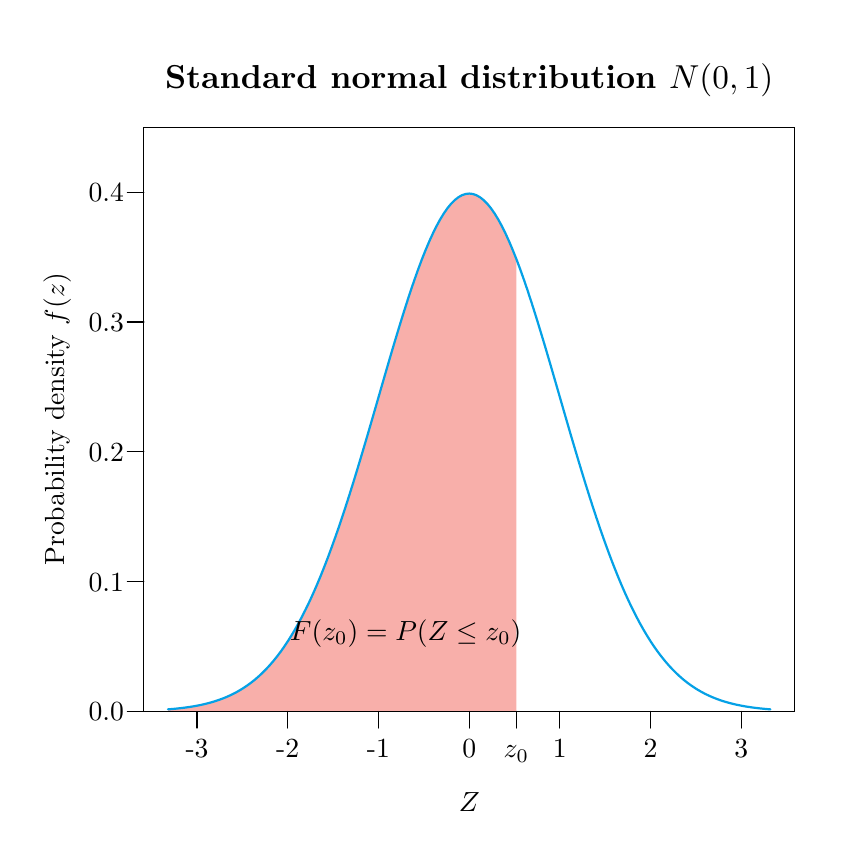
\begin{tikzpicture}[x=1pt,y=1pt]
  \definecolor{fillColor}{RGB}{255,255,255}
  \path[use as bounding box,fill=fillColor,fill opacity=0.00] (0,0) rectangle (289.08,289.08);
  \begin{scope}
  \path[clip] (  0.00,  0.00) rectangle (289.08,289.08);
  \definecolor{drawColor}{RGB}{0,0,0}
  
  \path[draw=drawColor,line width= 0.4pt,line join=round,line cap=round] ( 61.20, 42.00) -- (257.88, 42.00);
  
  \path[draw=drawColor,line width= 0.4pt,line join=round,line cap=round] ( 61.20, 42.00) -- ( 61.20, 36.00);
  
  \path[draw=drawColor,line width= 0.4pt,line join=round,line cap=round] ( 93.98, 42.00) -- ( 93.98, 36.00);
  
  \path[draw=drawColor,line width= 0.4pt,line join=round,line cap=round] (126.76, 42.00) -- (126.76, 36.00);
  
  \path[draw=drawColor,line width= 0.4pt,line join=round,line cap=round] (159.54, 42.00) -- (159.54, 36.00);
  
  \path[draw=drawColor,line width= 0.4pt,line join=round,line cap=round] (192.32, 42.00) -- (192.32, 36.00);
  
  \path[draw=drawColor,line width= 0.4pt,line join=round,line cap=round] (225.10, 42.00) -- (225.10, 36.00);
  
  \path[draw=drawColor,line width= 0.4pt,line join=round,line cap=round] (257.88, 42.00) -- (257.88, 36.00);
  
  \node[text=drawColor,anchor=base,inner sep=0pt, outer sep=0pt, scale=  1.00] at ( 61.20, 25.20) {-3};
  
  \node[text=drawColor,anchor=base,inner sep=0pt, outer sep=0pt, scale=  1.00] at ( 93.98, 25.20) {-2};
  
  \node[text=drawColor,anchor=base,inner sep=0pt, outer sep=0pt, scale=  1.00] at (126.76, 25.20) {-1};
  
  \node[text=drawColor,anchor=base,inner sep=0pt, outer sep=0pt, scale=  1.00] at (159.54, 25.20) {0};
  
  \node[text=drawColor,anchor=base,inner sep=0pt, outer sep=0pt, scale=  1.00] at (192.32, 25.20) {1};
  
  \node[text=drawColor,anchor=base,inner sep=0pt, outer sep=0pt, scale=  1.00] at (225.10, 25.20) {2};
  
  \node[text=drawColor,anchor=base,inner sep=0pt, outer sep=0pt, scale=  1.00] at (257.88, 25.20) {3};
  
  \path[draw=drawColor,line width= 0.4pt,line join=round,line cap=round] ( 42.00, 42.00) -- ( 42.00,229.63);
  
  \path[draw=drawColor,line width= 0.4pt,line join=round,line cap=round] ( 42.00, 42.00) -- ( 36.00, 42.00);
  
  \path[draw=drawColor,line width= 0.4pt,line join=round,line cap=round] ( 42.00, 88.91) -- ( 36.00, 88.91);
  
  \path[draw=drawColor,line width= 0.4pt,line join=round,line cap=round] ( 42.00,135.81) -- ( 36.00,135.81);
  
  \path[draw=drawColor,line width= 0.4pt,line join=round,line cap=round] ( 42.00,182.72) -- ( 36.00,182.72);
  
  \path[draw=drawColor,line width= 0.4pt,line join=round,line cap=round] ( 42.00,229.63) -- ( 36.00,229.63);
  
  \node[text=drawColor,anchor=base east,inner sep=0pt, outer sep=0pt, scale=  1.00] at ( 34.80, 38.56) {0.0};
  
  \node[text=drawColor,anchor=base east,inner sep=0pt, outer sep=0pt, scale=  1.00] at ( 34.80, 85.46) {0.1};
  
  \node[text=drawColor,anchor=base east,inner sep=0pt, outer sep=0pt, scale=  1.00] at ( 34.80,132.37) {0.2};
  
  \node[text=drawColor,anchor=base east,inner sep=0pt, outer sep=0pt, scale=  1.00] at ( 34.80,179.28) {0.3};
  
  \node[text=drawColor,anchor=base east,inner sep=0pt, outer sep=0pt, scale=  1.00] at ( 34.80,226.18) {0.4};
  
  \path[draw=drawColor,line width= 0.4pt,line join=round,line cap=round] ( 42.00, 42.00) --
    (277.08, 42.00) --
    (277.08,253.08) --
    ( 42.00,253.08) --
    ( 42.00, 42.00);
  \end{scope}
  \begin{scope}
  \path[clip] (  0.00,  0.00) rectangle (289.08,289.08);
  \definecolor{drawColor}{RGB}{0,0,0}
  
  \node[text=drawColor,anchor=base,inner sep=0pt, outer sep=0pt, scale=  1.20] at (159.54,266.94) {\bfseries Standard normal distribution $N(0,1)$};
  
  \node[text=drawColor,anchor=base,inner sep=0pt, outer sep=0pt, scale=  1.00] at (159.54,  6.00) {$Z$};
  
  \node[text=drawColor,rotate= 90.00,anchor=base,inner sep=0pt, outer sep=0pt, scale=  1.00] at ( 13.20,147.54) {Probability density $f(z)$};
  \end{scope}
  \begin{scope}
  \path[clip] (  0.00,  0.00) rectangle (289.08,289.08);
  \definecolor{drawColor}{RGB}{0,0,0}
  
  \path[draw=drawColor,line width= 0.4pt,line join=round,line cap=round] (176.59, 42.00) -- (176.59, 42.00);
  
  \path[draw=drawColor,line width= 0.4pt,line join=round,line cap=round] (176.59, 42.00) -- (176.59, 36.00);
  
  \node[text=drawColor,anchor=base,inner sep=0pt, outer sep=0pt, scale=  1.00] at (176.59, 25.20) {$z_0$};
  \end{scope}
  \begin{scope}
  \path[clip] ( 42.00, 42.00) rectangle (277.08,253.08);
  \definecolor{fillColor}{RGB}{238,50,36}
  
  \path[fill=fillColor,fill opacity=0.39] ( 50.71, 42.00) --
    ( 50.71, 42.76) --
    ( 52.02, 42.86) --
    ( 53.33, 42.98) --
    ( 54.64, 43.12) --
    ( 55.95, 43.27) --
    ( 57.26, 43.44) --
    ( 58.57, 43.63) --
    ( 59.89, 43.84) --
    ( 61.20, 44.08) --
    ( 62.51, 44.34) --
    ( 63.82, 44.63) --
    ( 65.13, 44.96) --
    ( 66.44, 45.32) --
    ( 67.75, 45.71) --
    ( 69.06, 46.15) --
    ( 70.38, 46.63) --
    ( 71.69, 47.16) --
    ( 73.00, 47.74) --
    ( 74.31, 48.37) --
    ( 75.62, 49.06) --
    ( 76.93, 49.82) --
    ( 78.24, 50.64) --
    ( 79.55, 51.54) --
    ( 80.87, 52.50) --
    ( 82.18, 53.55) --
    ( 83.49, 54.69) --
    ( 84.80, 55.91) --
    ( 86.11, 57.23) --
    ( 87.42, 58.64) --
    ( 88.73, 60.16) --
    ( 90.04, 61.78) --
    ( 91.36, 63.51) --
    ( 92.67, 65.36) --
    ( 93.98, 67.33) --
    ( 95.29, 69.41) --
    ( 96.60, 71.62) --
    ( 97.91, 73.96) --
    ( 99.22, 76.43) --
    (100.53, 79.03) --
    (101.85, 81.77) --
    (103.16, 84.63) --
    (104.47, 87.63) --
    (105.78, 90.76) --
    (107.09, 94.03) --
    (108.40, 97.42) --
    (109.71,100.95) --
    (111.02,104.59) --
    (112.34,108.35) --
    (113.65,112.23) --
    (114.96,116.22) --
    (116.27,120.30) --
    (117.58,124.48) --
    (118.89,128.75) --
    (120.20,133.09) --
    (121.51,137.49) --
    (122.83,141.94) --
    (124.14,146.44) --
    (125.45,150.96) --
    (126.76,155.50) --
    (128.07,160.04) --
    (129.38,164.56) --
    (130.69,169.05) --
    (132.00,173.50) --
    (133.32,177.88) --
    (134.63,182.19) --
    (135.94,186.40) --
    (137.25,190.50) --
    (138.56,194.48) --
    (139.87,198.30) --
    (141.18,201.97) --
    (142.49,205.47) --
    (143.81,208.77) --
    (145.12,211.87) --
    (146.43,214.74) --
    (147.74,217.39) --
    (149.05,219.79) --
    (150.36,221.94) --
    (151.67,223.82) --
    (152.98,225.43) --
    (154.30,226.75) --
    (155.61,227.79) --
    (156.92,228.53) --
    (158.23,228.98) --
    (159.54,229.13) --
    (160.85,228.98) --
    (162.16,228.53) --
    (163.47,227.79) --
    (164.78,226.75) --
    (166.10,225.43) --
    (167.41,223.82) --
    (168.72,221.94) --
    (170.03,219.79) --
    (171.34,217.39) --
    (172.65,214.74) --
    (173.96,211.87) --
    (175.27,208.77) --
    (176.59,205.47) --
    (176.59, 42.00) --
    cycle;
  \definecolor{drawColor}{RGB}{5,161,230}
  
  \path[draw=drawColor,line width= 0.8pt,line join=round,line cap=round] ( 50.71, 42.76) --
    ( 52.02, 42.86) --
    ( 53.33, 42.98) --
    ( 54.64, 43.12) --
    ( 55.95, 43.27) --
    ( 57.26, 43.44) --
    ( 58.57, 43.63) --
    ( 59.89, 43.84) --
    ( 61.20, 44.08) --
    ( 62.51, 44.34) --
    ( 63.82, 44.63) --
    ( 65.13, 44.96) --
    ( 66.44, 45.32) --
    ( 67.75, 45.71) --
    ( 69.06, 46.15) --
    ( 70.38, 46.63) --
    ( 71.69, 47.16) --
    ( 73.00, 47.74) --
    ( 74.31, 48.37) --
    ( 75.62, 49.06) --
    ( 76.93, 49.82) --
    ( 78.24, 50.64) --
    ( 79.55, 51.54) --
    ( 80.87, 52.50) --
    ( 82.18, 53.55) --
    ( 83.49, 54.69) --
    ( 84.80, 55.91) --
    ( 86.11, 57.23) --
    ( 87.42, 58.64) --
    ( 88.73, 60.16) --
    ( 90.04, 61.78) --
    ( 91.36, 63.51) --
    ( 92.67, 65.36) --
    ( 93.98, 67.33) --
    ( 95.29, 69.41) --
    ( 96.60, 71.62) --
    ( 97.91, 73.96) --
    ( 99.22, 76.43) --
    (100.53, 79.03) --
    (101.85, 81.77) --
    (103.16, 84.63) --
    (104.47, 87.63) --
    (105.78, 90.76) --
    (107.09, 94.03) --
    (108.40, 97.42) --
    (109.71,100.95) --
    (111.02,104.59) --
    (112.34,108.35) --
    (113.65,112.23) --
    (114.96,116.22) --
    (116.27,120.30) --
    (117.58,124.48) --
    (118.89,128.75) --
    (120.20,133.09) --
    (121.51,137.49) --
    (122.83,141.94) --
    (124.14,146.44) --
    (125.45,150.96) --
    (126.76,155.50) --
    (128.07,160.04) --
    (129.38,164.56) --
    (130.69,169.05) --
    (132.00,173.50) --
    (133.32,177.88) --
    (134.63,182.19) --
    (135.94,186.40) --
    (137.25,190.50) --
    (138.56,194.48) --
    (139.87,198.30) --
    (141.18,201.97) --
    (142.49,205.47) --
    (143.81,208.77) --
    (145.12,211.87) --
    (146.43,214.74) --
    (147.74,217.39) --
    (149.05,219.79) --
    (150.36,221.94) --
    (151.67,223.82) --
    (152.98,225.43) --
    (154.30,226.75) --
    (155.61,227.79) --
    (156.92,228.53) --
    (158.23,228.98) --
    (159.54,229.13) --
    (160.85,228.98) --
    (162.16,228.53) --
    (163.47,227.79) --
    (164.78,226.75) --
    (166.10,225.43) --
    (167.41,223.82) --
    (168.72,221.94) --
    (170.03,219.79) --
    (171.34,217.39) --
    (172.65,214.74) --
    (173.96,211.87) --
    (175.27,208.77) --
    (176.59,205.47) --
    (177.90,201.97) --
    (179.21,198.30) --
    (180.52,194.48) --
    (181.83,190.50) --
    (183.14,186.40) --
    (184.45,182.19) --
    (185.76,177.88) --
    (187.08,173.50) --
    (188.39,169.05) --
    (189.70,164.56) --
    (191.01,160.04) --
    (192.32,155.50) --
    (193.63,150.96) --
    (194.94,146.44) --
    (196.25,141.94) --
    (197.57,137.49) --
    (198.88,133.09) --
    (200.19,128.75) --
    (201.50,124.48) --
    (202.81,120.30) --
    (204.12,116.22) --
    (205.43,112.23) --
    (206.74,108.35) --
    (208.06,104.59) --
    (209.37,100.95) --
    (210.68, 97.42) --
    (211.99, 94.03) --
    (213.30, 90.76) --
    (214.61, 87.63) --
    (215.92, 84.63) --
    (217.23, 81.77) --
    (218.55, 79.03) --
    (219.86, 76.43) --
    (221.17, 73.96) --
    (222.48, 71.62) --
    (223.79, 69.41) --
    (225.10, 67.33) --
    (226.41, 65.36) --
    (227.72, 63.51) --
    (229.04, 61.78) --
    (230.35, 60.16) --
    (231.66, 58.64) --
    (232.97, 57.23) --
    (234.28, 55.91) --
    (235.59, 54.69) --
    (236.90, 53.55) --
    (238.21, 52.50) --
    (239.53, 51.54) --
    (240.84, 50.64) --
    (242.15, 49.82) --
    (243.46, 49.06) --
    (244.77, 48.37) --
    (246.08, 47.74) --
    (247.39, 47.16) --
    (248.70, 46.63) --
    (250.02, 46.15) --
    (251.33, 45.71) --
    (252.64, 45.32) --
    (253.95, 44.96) --
    (255.26, 44.63) --
    (256.57, 44.34) --
    (257.88, 44.08) --
    (259.19, 43.84) --
    (260.51, 43.63) --
    (261.82, 43.44) --
    (263.13, 43.27) --
    (264.44, 43.12) --
    (265.75, 42.98) --
    (267.06, 42.86) --
    (268.37, 42.76);
  \definecolor{drawColor}{RGB}{0,0,0}
  
  \node[text=drawColor,anchor=base,inner sep=0pt, outer sep=0pt, scale=  1.00] at (136.59, 67.64) {$F(z_0)=P(Z\leq z_0)$};
  \end{scope}
  \begin{scope}
  \path[clip] (  0.00,  0.00) rectangle (289.08,289.08);
  \definecolor{drawColor}{RGB}{0,0,0}
  
  \path[draw=drawColor,line width= 0.4pt,line join=round,line cap=round] ( 42.00, 42.00) --
    (277.08, 42.00) --
    (277.08,253.08) --
    ( 42.00,253.08) --
    ( 42.00, 42.00);
  \end{scope}
  \end{tikzpicture}
}
\end{center}

\begin{tabular}
{|r||r|r|r|r|r|r|r|r|r|r|}
\hline
\multicolumn{1}{|c||}{$\mathbf{z}$}&
\multicolumn{1}{c|}{\textbf{0,00}}&
\multicolumn{1}{c|}{\textbf{0,01}}&
\multicolumn{1}{c|}{\textbf{0,02}}&
\multicolumn{1}{c|}{\textbf{0,03}}&
\multicolumn{1}{c|}{\textbf{0,04}}&
\multicolumn{1}{c|}{\textbf{0,05}}&
\multicolumn{1}{c|}{\textbf{0,06}}&
\multicolumn{1}{c|}{\textbf{0,07}}&
\multicolumn{1}{c|}{\textbf{0,08}}&
\multicolumn{1}{c|}{\textbf{0,09}}\\
\hline\hline
\textbf{0,0}&
0,5000&
0,5040&
0,5080&
0,5120&
0,5160&
0,5199&
0,5239&
0,5279&
0,5319&
0,5359 \\
\hline
\textbf{0,1}&
0,5398&
0,5438&
0,5478&
0,5517&
0,5557&
0,5596&
0,5636&
0,5675&
0,5714&
0,5753 \\
\hline
\textbf{0,2}&
0,5793&
0,5832&
0,5871&
0,5910&
0,5948&
0,5987&
0,6026&
0,6064&
0,6103&
0,6141 \\
\hline
\textbf{0,3}&
0,6179&
0,6217&
0,6255&
0,6293&
0,6331&
0,6368&
0,6406&
0,6443&
0,6480&
0,6517 \\
\hline
\textbf{0,4}&
0,6554&
0,6591&
0,6628&
0,6664&
0,6700&
0,6736&
0,6772&
0,6808&
0,6844&
0,6879 \\
\hline
\textbf{0,5}&
0,6915&
0,6950&
0,6985&
0,7019&
0,7054&
0,7088&
0,7123&
0,7157&
0,7190&
0,7224 \\
\hline
\textbf{0,6}&
0,7257&
0,7291&
0,7324&
0,7357&
0,7389&
0,7422&
0,7454&
0,7486&
0,7517&
0,7549 \\
\hline
\textbf{0,7}&
0,7580&
0,7611&
0,7642&
0,7673&
0,7704&
0,7734&
0,7764&
0,7794&
0,7823&
0,7852 \\
\hline
\textbf{0,8}&
0,7881&
0,7910&
0,7939&
0,7967&
0,7995&
0,8023&
0,8051&
0,8078&
0,8106&
0,8133 \\
\hline
\textbf{0,9}&
0,8159&
0,8186&
0,8212&
0,8238&
0,8264&
0,8289&
0,8315&
0,8340&
0,8365&
0,8389 \\
\hline
\textbf{1,0}&
0,8413&
0,8438&
0,8461&
0,8485&
0,8508&
0,8531&
0,8554&
0,8577&
0,8599&
0,8621 \\
\hline
\textbf{1,1}&
0,8643&
0,8665&
0,8686&
0,8708&
0,8729&
0,8749&
0,8770&
0,8790&
0,8810&
0,8830 \\
\hline
\textbf{1,2}&
0,8849&
0,8869&
0,8888&
0,8907&
0,8925&
0,8944&
0,8962&
0,8980&
0,8997&
0,9015 \\
\hline
\textbf{1,3}&
0,9032&
0,9049&
0,9066&
0,9082&
0,9099&
0,9115&
0,9131&
0,9147&
0,9162&
0,9177 \\
\hline
\textbf{1,4}&
0,9192&
0,9207&
0,9222&
0,9236&
0,9251&
0,9265&
0,9279&
0,9292&
0,9306&
0,9319 \\
\hline
\textbf{1,5}&
0,9332&
0,9345&
0,9357&
0,9370&
0,9382&
0,9394&
0,9406&
0,9418&
0,9429&
0,9441 \\
\hline
\textbf{1,6}&
0,9452&
0,9463&
0,9474&
0,9484&
0,9495&
0,9505&
0,9515&
0,9525&
0,9535&
0,9545 \\
\hline
\textbf{1,7}&
0,9554&
0,9564&
0,9573&
0,9582&
0,9591&
0,9599&
0,9608&
0,9616&
0,9625&
0,9633 \\
\hline
\textbf{1,8}&
0,9641&
0,9649&
0,9656&
0,9664&
0,9671&
0,9678&
0,9686&
0,9693&
0,9699&
0,9706 \\
\hline
\textbf{1,9}&
0,9713&
0,9719&
0,9726&
0,9732&
0,9738&
0,9744&
0,9750&
0,9756&
0,9761&
0,9767 \\
\hline
\textbf{2,0}&
0,9772&
0,9778&
0,9783&
0,9788&
0,9793&
0,9798&
0,9803&
0,9808&
0,9812&
0,9817 \\
\hline
\textbf{2,1}&
0,9821&
0,9826&
0,9830&
0,9834&
0,9838&
0,9842&
0,9846&
0,9850&
0,9854&
0,9857 \\
\hline
\textbf{2,2}&
0,9861&
0,9864&
0,9868&
0,9871&
0,9875&
0,9878&
0,9881&
0,9884&
0,9887&
0,9890 \\
\hline
\textbf{2,3}&
0,9893&
0,9896&
0,9898&
0,9901&
0,9904&
0,9906&
0,9909&
0,9911&
0,9913&
0,9916 \\
\hline
\textbf{2,4}&
0,9918&
0,9920&
0,9922&
0,9925&
0,9927&
0,9929&
0,9931&
0,9932&
0,9934&
0,9936 \\
\hline
\textbf{2,5}&
0,9938&
0,9940&
0,9941&
0,9943&
0,9945&
0,9946&
0,9948&
0,9949&
0,9951&
0,9952 \\
\hline
\textbf{2,6}&
0,9953&
0,9955&
0,9956&
0,9957&
0,9959&
0,9960&
0,9961&
0,9962&
0,9963&
0,9964 \\
\hline
\textbf{2,7}&
0,9965&
0,9966&
0,9967&
0,9968&
0,9969&
0,9970&
0,9971&
0,9972&
0,9973&
0,9974 \\
\hline
\textbf{2,8}&
0,9974&
0,9975&
0,9976&
0,9977&
0,9977&
0,9978&
0,9979&
0,9979&
0,9980&
0,9981 \\
\hline
\textbf{2,9}&
0,9981&
0,9982&
0,9982&
0,9983&
0,9984&
0,9984&
0,9985&
0,9985&
0,9986&
0,9986 \\
\hline
\textbf{3,0}&
0,9987&
0,9987&
0,9987&
0,9988&
0,9988&
0,9989&
0,9989&
0,9989&
0,9990&
0,9990 \\
\hline
\textbf{3,1}&
0,9990&
0,9991&
0,9991&
0,9991&
0,9992&
0,9992&
0,9992&
0,9992&
0,9993&
0,9993 \\
\hline
\textbf{3,2}&
0,9993&
0,9993&
0,9994&
0,9994&
0,9994&
0,9994&
0,9994&
0,9995&
0,9995&
0,9995 \\
\hline
\textbf{3,3}&
0,9995&
0,9995&
0,9995&
0,9996&
0,9996&
0,9996&
0,9996&
0,9996&
0,9996&
0,9997 \\
\hline
\textbf{3,4}&
0,9997&
0,9997&
0,9997&
0,9997&
0,9997&
0,9997&
0,9997&
0,9997&
0,9997&
0,9998 \\
\hline
\end{tabular}
\end{center}

\end{document}
